\scanpage{4}
\mspage{\handwritten{(30}}
\begingroup
\reversemarginpar
\makeatletter\tagsleft@true\makeatother
\noindent\margin{\handwritten{$\varphi\qquad \varepsilon_{\xi'}$}}%
\handwritten{\tikz[baseline=-.2ex]{\draw (0,0) .. controls (.13,.16) and (.36,.24) .. (.43,.21) .. controls (.45,.19) and (.45,.17) .. (.45,.16);}}\,
When $\handwritten{\varphi}$ is of the form $\handwritten{\varepsilon_{\xi'\raisebox{.45ex}{$\scriptstyle\deleted{\unsure{\xi'|\xi}}$}}}$, hence
\margin{\handwritten{$\varphi$}}
\[
\handwritten{\varphi} \handwritten{\simeq} \mathop{\underset{\handwritten{\longrightarrow}}{\mathrm{lim}}}\limits_j {X'_j}^{\handwritten{\unsure{\vee|v}}}\ , 
\]
we therefore have a natural bijection
\margin{\handwritten{$\varepsilon_{\xi}\quad\varepsilon_{\xi'}\qquad .$}}
\[
\operatorname{Hom}\bigl(\handwritten{\varepsilon_{\substack{\deleted{\unsure{\xi}}\\[-.4ex]\xi}}},\handwritten{\varepsilon_{\substack{\deleted{\unsure{\xi}}\\[-.4ex]\xi\unsure{'}}}} ,\bigr)
 \handwritten{\simeq} \mathop{\underset{\handwritten{\longleftarrow}}{\mathrm{lim}}}\limits_i \mathop{\underset{\handwritten{\longrightarrow}}{\mathrm{lim}}}\limits_j \operatorname{Hom}_{X}(X'_j,X_i)\handwritten{\deleted{\unsure{,|.}}}\qquad .
\tag*{$(*)$}
\]

\noindent On the other hand we have (in the category of preschemes)
\margin{\handwritten{$\deleted{\unsure{\xi}}$}}
\[
\bar X(\handwritten{\xi}) == \mathop{\underset{\handwritten{\longleftarrow}}{\mathrm{lim}}}\limits_i X_i\handwritten{\deleted{\xi}}\ ,\quad
\bar X(\handwritten{\xi}') = \mathop{\underset{\handwritten{\longleftarrow}}{\mathrm{lim}}}\limits_j X'_j\ ,
\]
whence
\[
\handwritten{\tikz[baseline=-.2ex]{\draw (0,0) .. controls (.08,-.03) and (.18,.03) .. (.23,.08);}}\; \operatorname{Hom}_{X}(\bar X(\handwritten{\xi}'),\bar X(\handwritten{\xi})) \handwritten{\simeq}
 \mathop{\underset{\handwritten{\longleftarrow}}{\mathrm{lim}}}\limits_i \operatorname{Hom}_{X}(\bar X(\handwritten{\xi}'),X_i)\ ,
\]
\margin{\handwritten{\tikz{\draw (0,0) .. controls (.04,.18) and (.27,.10) .. (.49,.28) .. controls (.58,.35) and (.56,.45) .. (.54,.47);}}}
on the other hand, since $X_i$ is loc\inserted{\handwritten{\tikz[baseline=(w.base)]{%
\node[anchor=base west,rotate=14,inner sep=.3pt] (w) at (0,0) {ally};
\draw (-.04,-.17) .. controls (-.01,.08) and (.42,.04) .. (.85,.27) .. controls (.98,.34) and (1.04,.41) .. (.99,.42);
}}} of finite presentation over $X$\handwritten{, we have}
\[
\operatorname{Hom}_{\handwritten{X}}(\bar X(\handwritten{\xi}'),X_i) \handwritten{\simeq}
 \mathop{\underset{\handwritten{\longrightarrow}}{\mathrm{lim}}}\limits_j \operatorname{Hom}_{X}(X_j,X_i)\handwritten{,}
\]
whence
\[
\operatorname{Hom}_{X}(\bar X(\handwritten{\xi}'),\bar X(\handwritten{\xi})) \handwritten{\simeq}
 \mathop{\underset{\handwritten{\longleftarrow}}{\mathrm{lim}}}\limits_i \mathop{\underset{\handwritten{\longrightarrow}}{\mathrm{lim}}}\limits_j \operatorname{Hom}_{X}(X'_j,X_i)\ .
\tag*{$(**)$}
\]

\noindent The comparison of $(*)$ is $(**)$ gives the\handwritten{$\mid$}desired conclusion (subject to a verification of compatibilities, lef\deleted{\unsure{n|e|s}}t to the reader).

% slanted
\noindent\margin{\handwritten{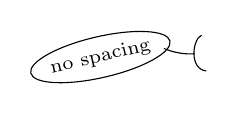
\begin{tikzpicture}[baseline,scale=.84]
\node[rotate=13,inner sep=1pt] (m) at (0,0) {\scriptsize\unsure{no} spacing};
\draw[rotate=13] (0,0) ellipse [x radius=1.08cm,y radius=.31cm];
\draw (.96,.13) .. controls (1.13,.06) and (1.29,.04) .. (1.42,.05);
\draw (1.53,.33) .. controls (1.39,.27) and (1.34,-.18) .. (1.60,-.21);
\end{tikzpicture}}}%
b) \uline{The functor under consideration is essentially surjective:}

\noindent 7.9.1.\quad Let us first note that if $C$ is a site where finite $\mathop{\underset{\handwritten{\longleftarrow}}{\mathrm{lim}}}\limits$ are representable, $\handwritten{\widetilde}{C} = \underline{E}$ the corresponding topos then\handwritten{,} \deleted{all}\handwritten{every}%
\margin{\handwritten{,\quad t}}
fiber\deleted{s} functor\deleted{s} $\handwritten{\overset{\deleted{\unsure{\varphi|\xi}}}{\varphi}}$ on $\underline E$ can be represented as a
\margin{\handwritten{$/\quad /\quad\varphi$}}
connecte\deleted{\unsure{d}}\handwritten{d} pseudo-filtering inductive ``limit''\handwritten{''} o\deleted{f}\handwritten{f} functors of the form
\margin{\handwritten{e\quad e}}
\margin{\handwritten{$]\,[ $}}
\[
\handwritten{\check}{Y}(F) == F(Y) = \operatorname{Hom}(\handwritten{\widetilde}{Y},F),\handwritten{\big]\big[}\, Y\handwritten{\in}\operatorname{Ob} C\handwritten{,}
\]
(where $\handwritten{\widetilde}{Y}$ is the sheaf associated to $Y$)\handwritten{,} in the following way. We consid\deleted{\unsure{er|er}}\handwritten{er}
\margin{\handwritten{,}}
the category\handwritten{$\mid C_{\substack{\deleted{\unsure{\xi|\varphi}}\\[-.4ex]\varphi}}$} of pairs $(Y,\handwritten{\xi})$, with $Y\handwritten{\in}\operatorname{Ob} C$, $\handwritten{\xi}\handwritten{\in\varphi}(\handwritten{\widetilde}{Y})$
\margin{\handwritten{$C_{\varphi}$}}
\endgroup

% archive sheet number: 3
\clearpage
